\section{Fonction}

Comme expliqué dans l'introduction, les filtres servent à limiter
le domaine de fréquences du signal à un certain intervalle
$[f\ind{bas},f\ind{haut}]$.
Les fréquences situées en-dehors de cet intervalle seront atténuées,
comme l'illustre la figure~\ref{fig:filtre-ideal} en échelle log-log.

\begin{figure}[h!]
    \centering
    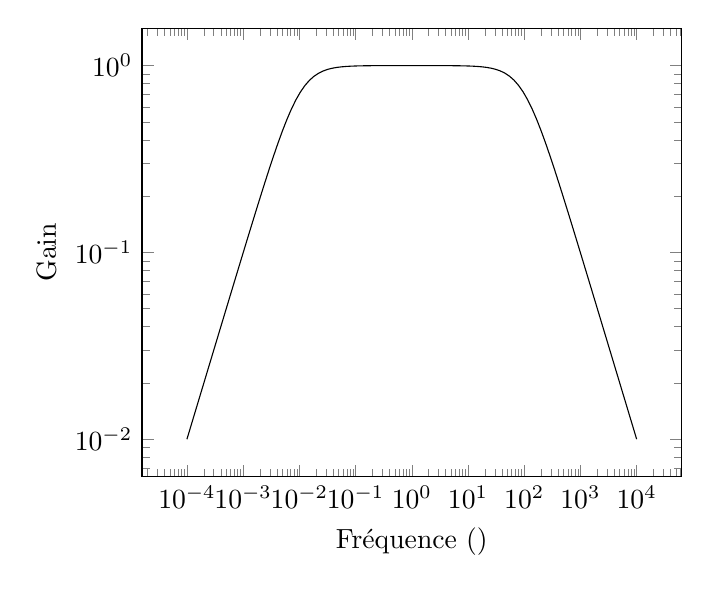
\begin{tikzpicture}
        \begin{loglogaxis}[
                xlabel={Fréquence (\hertz)},
                ylabel={Gain},
            ]
            \addplot[domain=1e-4:1e4,samples=100]
            {1 / sqrt(1+1/(10000*x^2)) / sqrt(1+x^2/10000)};
        \end{loglogaxis}
    \end{tikzpicture}
    \caption{Filtre passe-bande --- ici, $f\ind{bas}=10^{-2}$, $f\ind{haut}=10^2$}
    \label{fig:filtre-ideal}
\end{figure}

Ce genre de dispositif s'appelle un filtre \emph{passe-bande},
car il tend à laisser passer une bande de fréquences et exclure le reste.
\cite{highpass-def}
Il peut être formé par la combinaison d'un filtre
\emph{passe-haut} et d'un filtre \emph{passe-bas}, \cite{high-low-pass-combined}
comme c'est le cas dans notre circuit.

En particulier,
le filtre \emph{passe-haut} laisse passer les hautes fréquences,
il se charge donc d'atténuer les basses fréquences ($f<f\ind{bas}$);
tandis que le filtre \emph{passe-bas} laisse passer les basses fréquences,
il se charge donc d'atténuer les hautes fréquences ($f>f\ind{haut}$).

Pour se donner une idée,
l'oreille humaine est capable de percevoir des sons de fréquences
allant de $20\,\hertz$ à $20\,\kilo\hertz$. \cite{hearing-range}
En musique, les basses fréquences correspondent aux notes graves et aux basses,
tandis que les hautes fréquences correspondent aux notes aiguës et
à la mélodie.

Par conséquent, une première fonction des filtres est de
favoriser la mélodie au détriment des
basses, ou les basses au détriment de la mélodie, selon les préférences
de l'auditeur.

De plus, étant donné la grande étendue des fréquences audibles,
une deuxième fonction possible est de séparer les graves des aigus
afin de les diffuser par deux haut-parleurs spécialisés chacun
dans la restitution de sa bande de fréquences,
comme nous avons décidé de le faire lors de ce projet.
